% Created 2017-11-11 Sat 19:25
% Intended LaTeX compiler: pdflatex
\documentclass[titlepage]{article}
\usepackage[utf8]{inputenc}
\usepackage[T1]{fontenc}
\usepackage{graphicx}
\usepackage{grffile}
\usepackage{longtable}
\usepackage{wrapfig}
\usepackage{rotating}
\usepackage[normalem]{ulem}
\usepackage{amsmath}
\usepackage{textcomp}
\usepackage{amssymb}
\usepackage{capt-of}
\usepackage{hyperref}
\hypersetup{hidelinks=true}
\setlength{\parindent}{2em}
\usepackage[margin=1in]{geometry}
\author{Hu Xiaoxiang \\
U1521319A \\
EEE \\
}
\date{11 Nov, 2017 \\
}
\title{
\includegraphics[width=\textwidth]{logo_ntu_new.png} \\
[5\baselineskip] FYP \\
INTERIM \\
REPORT \\
[5\baselineskip]}
\hypersetup{
 pdfauthor={Hu Xiaoxiang \\
U1521319A \\
EEE \\
},
 pdftitle={
\includegraphics[width=\textwidth]{logo_ntu_new.png} \\
[5\baselineskip] FYP \\
INTERIM \\
REPORT \\
[5\baselineskip]},
 pdfkeywords={},
 pdfsubject={},
 pdfcreator={Emacs 25.1.1 (Org mode 9.1.2)}, 
 pdflang={English}}
\begin{document}

\maketitle
\tableofcontents

\pagenumbering{roman}
\newpage
\pagenumbering{arabic}

\section{Introduction}
\label{sec:org4837838}
Object detection is a technology related to computer vision and image
processing. In terms of algorithm, classical techniques, including point
processing, edge detection and morphological operation, can be used to detect
objects edge of a certain class(such as humans, buildings or cars) in digital
images and videos. With the development of deep learning in recent years, new
techniques such as Convolutional Neural Network(CNN) appears to show its high
accuracy on object detection task.

The objective of my project is to apply deep learning techniques on object
detection in auto driving environment. The deep learning techniques include
Extreme Learning Machine(ELM), CNN, and so on. By the end of this project, it
is supposed to demonstrate a deep neural network which should have capability
to differentiate object such as vehicles, bicycle riders and pedestrians.

\section{Research Progress}
\label{sec:org1bc5191}
Object detection can use both classical method and deep learning method. Each
of them has its own advantages and disadvantages. Typically, the classical
method is used as a pre-processing procedure for noise removal, contrast
enhancement or image segmentation. Especially, the pre-processing method can
be used for data augmentation to mend some overfitting problems, which is
usually caused by having too few samples for model to learn from. On the other
side, deep learning method has its advantages on feature engineering over
classical method. Shortly speaking, a deep neural network can learn object's
features by itself, which is a very essential characteristic for object
detection in auto driving environment, because the complexity of image
features usually can become too high so that classical algorithm cannot handle
it both efficiently and accurately. In order to utilize the advantages of both
sides, the range of my first-stage research covers these two fields:

\begin{enumerate}
\item Fundamentals of deep learning techniques and the utilization of mature deep
learning framework, such as using TensorFlow as backend and Keras as front end.
\item Computer vision basic and practical exercise using computer vision tools,
such as OpenCV.
\end{enumerate}

\subsection{Deep Learning Field}
\label{sec:org47aef59}
\begin{figure}[htbp]
\centering
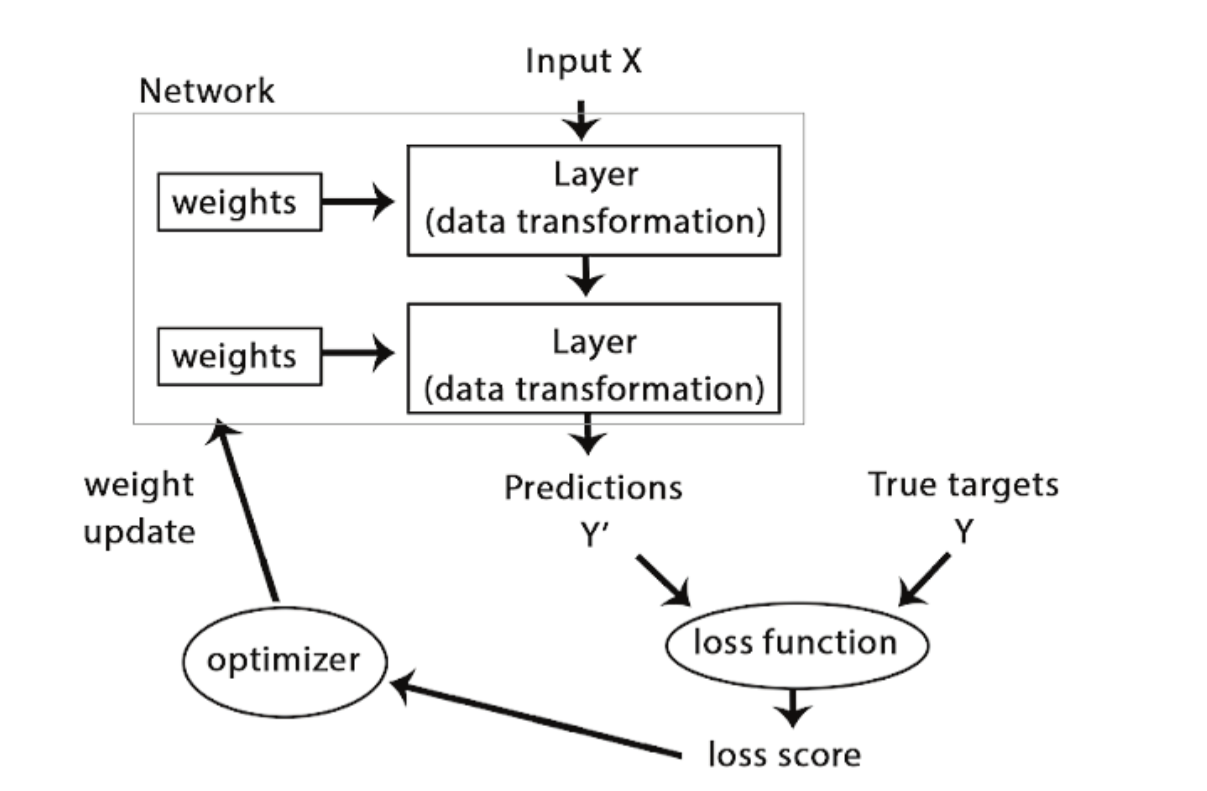
\includegraphics[width=300]{cnn_model.PNG}
\caption{Neural Network Model}
\end{figure}
\newpage

The major deep learning technique I researched for the first stage is CNN.
The core building block of CNN is the "layer". The layer is a data-processing
module which can be conceived as a "filter" for data. It extracts
representations or features out of the data fed into them. These
representations determine the weight of nodes within each layers. The weight
of nodes changes dynamically after each iteration of learning progress,
according to both value of input and difference between output and target
value, which is also known as the loss score. To update the weight on each
node, the CNN use "backpropagation" algorithm.

\begin{listing}
\begin{verbatim}
from keras import layers
from keras import models
from keras import optimizers

model = models.Sequential()
model.add(layers.Conv2D(32, (3, 3), activation='relu',
                        input_shape=(150, 150, 3)))
model.add(layers.MaxPooling2D((2, 2)))
model.add(layers.Conv2D(64, (3, 3), activation='relu'))
model.add(layers.MaxPooling2D((2, 2)))
model.add(layers.Conv2D(128, (3, 3), activation='relu'))
model.add(layers.MaxPooling2D((2, 2)))
model.add(layers.Conv2D(128, (3, 3), activation='relu'))
model.add(layers.MaxPooling2D((2, 2)))
model.add(layers.Flatten())
model.add(layers.Dense(512, activation='relu'))
model.add(layers.Dense(1, activation='sigmoid'))

model.compile(loss='binary_crossentropy',
              optimizer=optimizers.RMSprop(lr=1e-4),
              metrics=['acc'])
\end{verbatim}
\centering
\caption{List 1: Use Keras creating CNN model}
\newline
\end{listing}

The CNN framework in TensorFlow and Keras consists of two main layers, which
are convolution layers and pooling layers. The fundamental difference between
a normal densely-connected layer and a convolution layer is this: dense
layers learn global patterns in their input feature space, while convolution
layers learn local patterns through a convolution kernel. Due to this
characteristic, the patterns CNN learns are translation-invariant. Unlike
convolution layers splitting entire image into many small features, the role
of pooling layers is to aggressively downsample feature maps. By doing this,
it allows successive convolution layers to learn spatial hierarchies of
patterns through increasingly large window and hence reduce the influence of
overfitting [1].

Known the fundamental component of CNN, what I have exercised is to use a
pre-trained model, which is trained by Microsoft Common Objects in Context
(COCO) dataset, to detect the bicycle rider on images. The purpose of using a
pre-trained model is that it can help to reduce the training time
significantly and meanwhile maintain a high accuracy on validation set even
given small number of training samples.

To train a CNN model using TensorFlow backend, it needs to prepare some
labeled training data. What I tried is to download pictures directly from
google image search engine by using a image crawler. One of the benefits is
that it helps to degrade the resolution of images to a level of 200 x 150
pixels, which is exactly a suitable size for deep neural network when the
amount of training data is huge.

\begin{listing}
\begin{verbatim}
# Command for fetch urls from google image search on chrome:
# a = document.querySelectorAll('img')
# document.body.innerText = Array.prototype.map.call(a,x=>x.currentSrc)

import os
import re
import urllib.request

root_path = os.path.abspath('~/Documents/images/')
object_class = 'car'
object_path = 'img_'+object_class

url_path = os.path.join(root_path, object_path, object_class+'URL.txt')

result = []
with open(url_path, 'r') as file:
    while True:
        line = file.read(1024)
        if not line:
            break
        a = line.split(',')
        for i in a:
            item = re.match('^https', i)
            if item is not None:
                result.append(i.strip())
n=0
for url in result:
    try:
        figure_name = ''.join([object_class, '_fig_', str(n), '.jpg'])
        figure_path = os.path.join(root_path, object_path,figure_name)
        urllib.request.urlretrieve(url,figure_path)
        n += 1
    except:
        pass
\end{verbatim}
\centering
\caption{List 2: Image Crawler}
\newline
\end{listing}

The next step is to label the training images. The tool I used for image
labeling is called "labelImg" [2] (Figure 2). Basically, this tool helps to
generate a ".xml" file to store the label tag (List 3).

\begin{figure}[htbp]
\centering
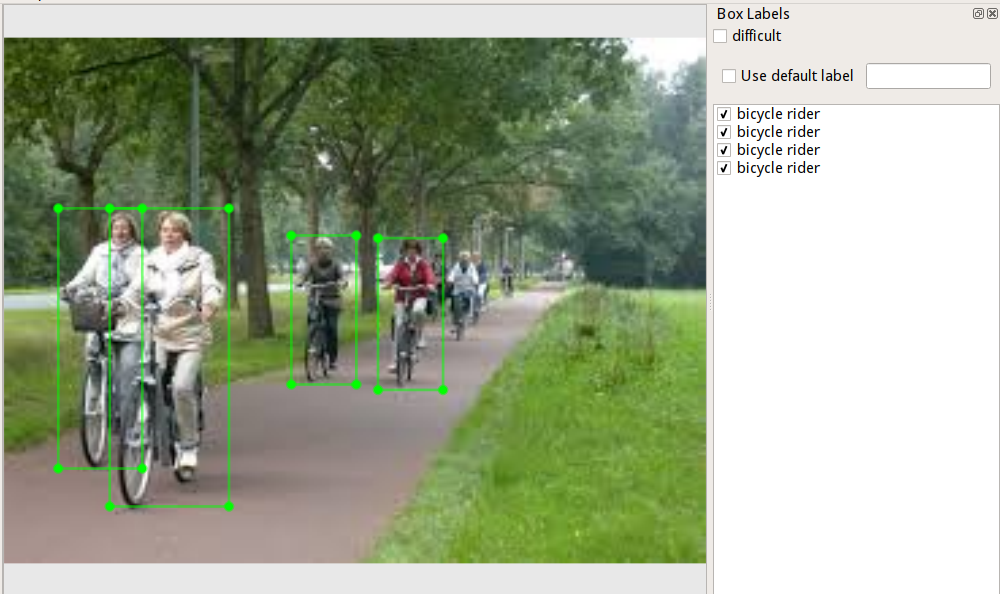
\includegraphics[width=300]{img_labeling.png}
\caption{Labeled Image}
\end{figure}

\begin{listing}
\begin{verbatim}
<annotation>
  <folder>img_bicycle</folder>
  <filename>bicycle_fig_1.jpg</filename>
  <path>/home/seanhxx/Documents/images/img_bicycle/bicycle_fig_1.jpg</path>
  <source>
    <database>Unknown</database>
  </source>
  <size>
    <width>275</width>
    <height>183</height>
    <depth>3</depth>
  </size>
  <segmented>0</segmented>
  <object>
    <name>bicycle rider</name>
    <pose>Unspecified</pose>
    <truncated>0</truncated>
    <difficult>0</difficult>
    <bndbox>
      <xmin>85</xmin>
      <ymin>15</ymin>
      <xmax>257</xmax>
      <ymax>173</ymax>
    </bndbox>
  </object>
</annotation>
\end{verbatim}
\centering
\caption{List 3: Label Infomation}
\newline
\end{listing}

The final step of training data preparation is to generate a
TensorFlow-recognizable data record [3] (List 4). The number of training
dataset I used here is 150 and validation data set is 16.

\begin{listing}
\begin{verbatim}
def create_tf_example(group, path):
    with tf.gfile.GFile(os.path.join(path, '{}'.format(group.filename)), 'rb') as fid:
        encoded_jpg = fid.read()
    encoded_jpg_io = io.BytesIO(encoded_jpg)
    image = Image.open(encoded_jpg_io)
    width, height = image.size

    filename = group.filename.encode('utf8')
    image_format = b'jpg'
    xmins = []
    xmaxs = []
    ymins = []
    ymaxs = []
    classes_text = []
    classes = []

    for index, row in group.object.iterrows():
        xmins.append(row['xmin'] / width)
        xmaxs.append(row['xmax'] / width)
        ymins.append(row['ymin'] / height)
        ymaxs.append(row['ymax'] / height)
        classes_text.append(row['class'].encode('utf8'))
        classes.append(class_text_to_int(row['class']))

    tf_example = tf.train.Example(features=tf.train.Features(feature={
        'image/height': dataset_util.int64_feature(height),
        'image/width': dataset_util.int64_feature(width),
        'image/filename': dataset_util.bytes_feature(filename),
        'image/source_id': dataset_util.bytes_feature(filename),
        'image/encoded': dataset_util.bytes_feature(encoded_jpg),
        'image/format': dataset_util.bytes_feature(image_format),
        'image/object/bbox/xmin': dataset_util.float_list_feature(xmins),
        'image/object/bbox/xmax': dataset_util.float_list_feature(xmaxs),
        'image/object/bbox/ymin': dataset_util.float_list_feature(ymins),
        'image/object/bbox/ymax': dataset_util.float_list_feature(ymaxs),
        'image/object/class/text': dataset_util.bytes_list_feature(classes_text),
        'image/object/calass/label': dataset_util.int64_list_feature(classes),
    }))
    return tf_example
\end{verbatim}
\centering
\caption{List 4: Generate TensorFlow Record}
\newline
\end{listing}

After the training data is prepared, the execution of following procedures
will feed data into the neural network. As what I mentioned before, to reduce
training time and increase accuracy with small amount of training data, a
pre-trained model is used at current stage of research. Besides, TensorFlow
Object Detection API provides the function to train a pre-trained model with
new data set [5]. The total loss of validation is shown in Figure 3.

\begin{figure}[htbp]
\centering
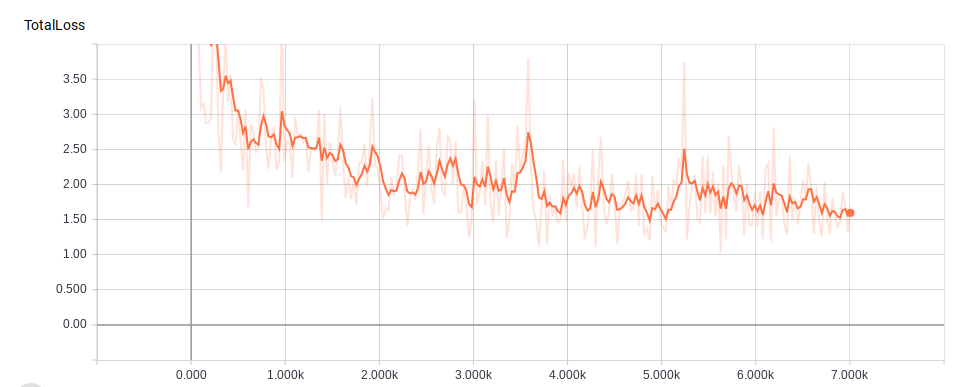
\includegraphics[width=300]{total_loss.png}
\caption{Total Loss Of Validation}
\end{figure}

As shown in Figure 4 and 5, the test images show the percentage of
reliability of the detection. Due to the limit amount of training data, the
loss is relatively high, and occasionally some test images actually cannot be
recognized even. To solve this overfitting problem, image processing
techniques are needed for data augmentation.

\begin{figure}[htbp]
\centering
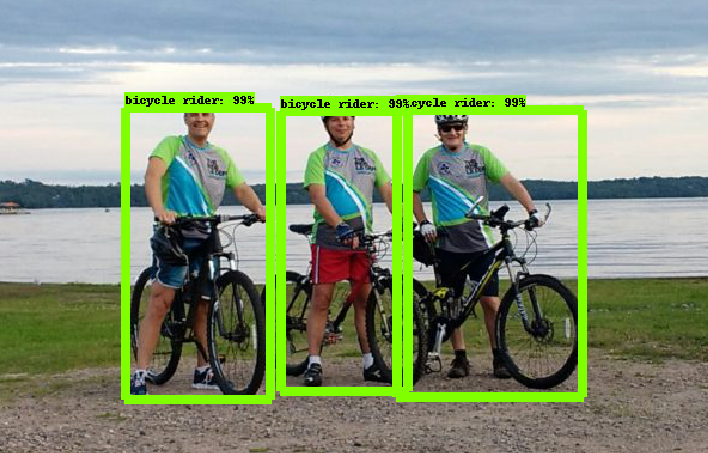
\includegraphics[width=200]{test1.png}
\caption{Test Result 1}
\end{figure} 

\newpage
\begin{figure}[htbp]
\centering
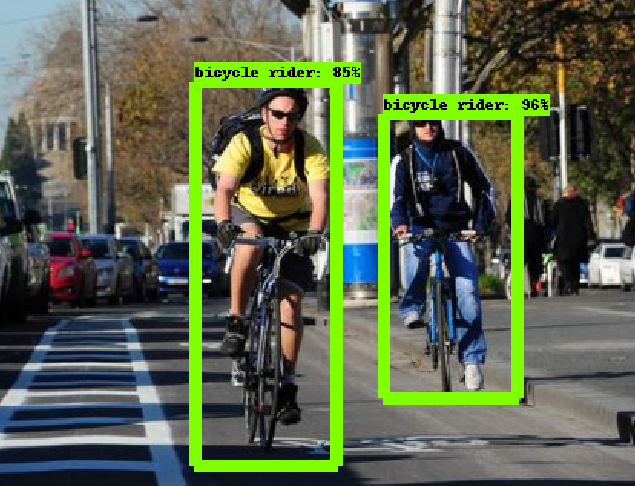
\includegraphics[width=200]{test2.png}
\caption{Test Result 2}
\end{figure}

\subsection{Computer Vision Field}
\label{sec:org56be481}
The research target on computer vision field for the first semester is to
learn some basic image processing techniques and use openCV via python
API. 

To reduce the calculation cost, a color image is typically converted to
a gray scale image before fed into deep neural network. To reduce the noise,
Gaussian filter or alpha-trimmed mean filter can be applied. Point processing
tools like contrast stretching is used to improve the illumination of images
which are under exposure. As what I mentioned before, image transformation or
degradation function can also be used for data augmentation to mitigate
overfitting problem. 

\begin{figure}[htbp]
\centering
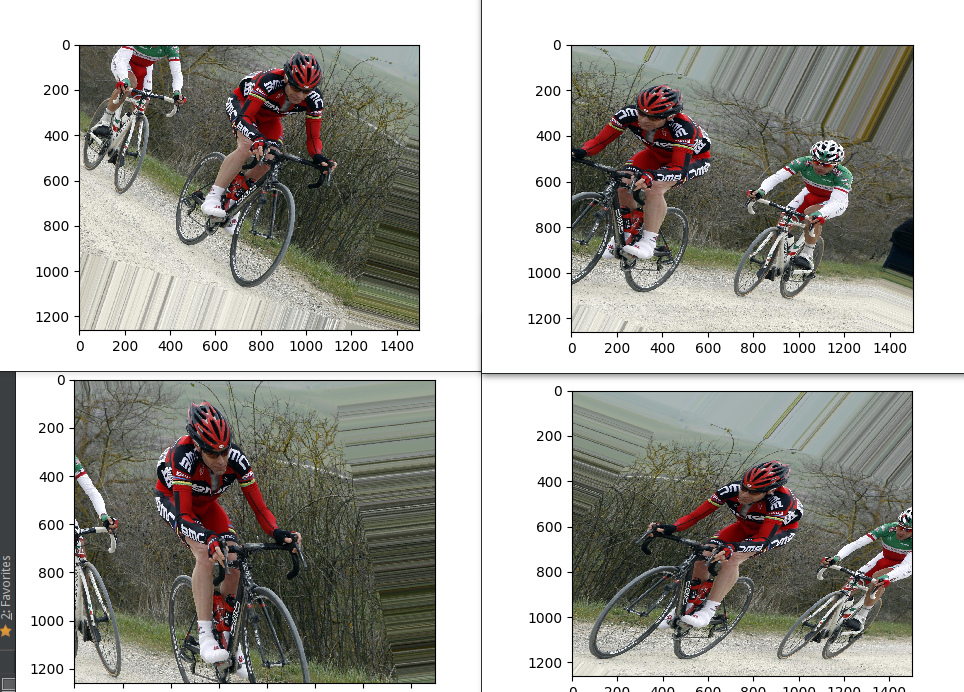
\includegraphics[width=300]{data_aug.png}
\caption{Data Augmentation}
\end{figure}

OpenCV is a open source computer vision library and provides plenty of
embedded computer vision functions for immediate use. When compiling OpenCV
with python binding, one can use OpenCV python API to control camera devices on
different hardwares. For example, the web camera on laptop can be accessed
directly through python and can be used as a testing of the pre-trained model at
real time (Figure 6).

\begin{figure}[htbp]
\centering
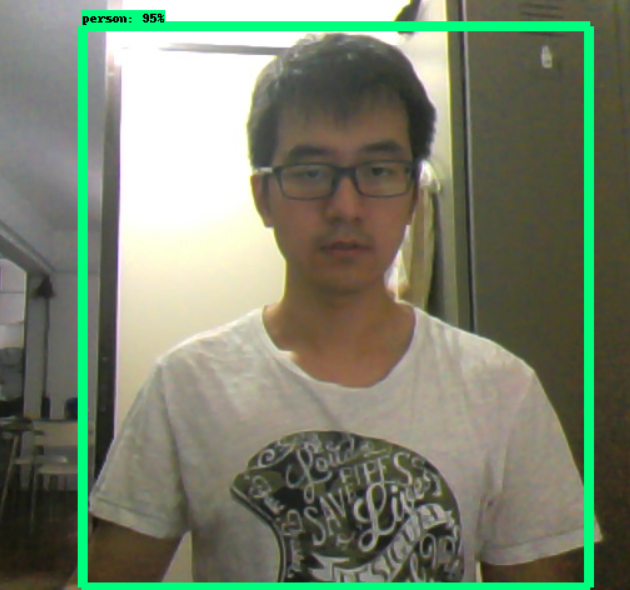
\includegraphics[width=200]{openCV.png}
\caption{Real Time Object Detection}
\end{figure}
\newpage

\section{Plan For Next Stage}
\label{sec:org46c1947}
Based on my current research progress, the plan for the next step is to study
and try to implement one of the state-of-the-art deep learning techniques,
such as CNN-ELM and Mask R-CNN. Another potential research direction is about
applying Recursive Cortical Network (RCN) [4] on object detection area.
Currently, CNN can achieve a good accuracy on object detection task with
enough number of lossless training samples. However, in a real time world like
auto driving environment, it is impossible to collect images of street view
under different situations with a perfect quality all the time. Moreover,
image pre-processing and long training time required by CNN also limit its
application on auto driving environment. To solve this problem, a new neural
network RCN, which mimics human brain's cortex and has already achieved high
accuracy on CAPTCHA recognition, may be used for general object detection.


\addcontentsline{toc}{section}{References}

\begin{thebibliography}{5}

\bibitem{1}Chollet, F. (2017). Deep Learning With Python. 1st ed. Manning Pubns Co, pp. 111-112

\bibitem{2}\textsc{GitHub} (2017) LabelImg [online] Available at: https://github.com/tzutalin/labelImg

\bibitem{3}\textsc{Learning Python} (2017) Object Detection [online] Available at: https://pythonprogramming.net/

\bibitem{4}\textsc{Vicarious} (2017) Common Sense, Cortex, and CAPTCHA
\newline
[online] Available at: https://www.vicarious.com/2017/10/26/common-sense-cortex-and-captcha/ 

\bibitem{5}\textsc{TensorFlow} (2017) TensorFlow Object Detection API 
\newline
[online] Available at: https://github.com/tensorflow/models/tree/master/research/object_detection


\end{thebibliography}
\end{document}
